\documentclass[twoside]{book}

% Packages required by doxygen
\usepackage{fixltx2e}
\usepackage{calc}
\usepackage{doxygen}
\usepackage[export]{adjustbox} % also loads graphicx
\usepackage{graphicx}
\usepackage[utf8]{inputenc}
\usepackage{makeidx}
\usepackage{multicol}
\usepackage{multirow}
\PassOptionsToPackage{warn}{textcomp}
\usepackage{textcomp}
\usepackage[nointegrals]{wasysym}
\usepackage[table]{xcolor}

% Font selection
\usepackage[T1]{fontenc}
\usepackage[scaled=.90]{helvet}
\usepackage{courier}
\usepackage{amssymb}
\usepackage{sectsty}
\renewcommand{\familydefault}{\sfdefault}
\allsectionsfont{%
  \fontseries{bc}\selectfont%
  \color{darkgray}%
}
\renewcommand{\DoxyLabelFont}{%
  \fontseries{bc}\selectfont%
  \color{darkgray}%
}
\newcommand{\+}{\discretionary{\mbox{\scriptsize$\hookleftarrow$}}{}{}}

% Page & text layout
\usepackage{geometry}
\geometry{%
  a4paper,%
  top=2.5cm,%
  bottom=2.5cm,%
  left=2.5cm,%
  right=2.5cm%
}
\tolerance=750
\hfuzz=15pt
\hbadness=750
\setlength{\emergencystretch}{15pt}
\setlength{\parindent}{0cm}
\setlength{\parskip}{3ex plus 2ex minus 2ex}
\makeatletter
\renewcommand{\paragraph}{%
  \@startsection{paragraph}{4}{0ex}{-1.0ex}{1.0ex}{%
    \normalfont\normalsize\bfseries\SS@parafont%
  }%
}
\renewcommand{\subparagraph}{%
  \@startsection{subparagraph}{5}{0ex}{-1.0ex}{1.0ex}{%
    \normalfont\normalsize\bfseries\SS@subparafont%
  }%
}
\makeatother

% Headers & footers
\usepackage{fancyhdr}
\pagestyle{fancyplain}
\fancyhead[LE]{\fancyplain{}{\bfseries\thepage}}
\fancyhead[CE]{\fancyplain{}{}}
\fancyhead[RE]{\fancyplain{}{\bfseries\leftmark}}
\fancyhead[LO]{\fancyplain{}{\bfseries\rightmark}}
\fancyhead[CO]{\fancyplain{}{}}
\fancyhead[RO]{\fancyplain{}{\bfseries\thepage}}
\fancyfoot[LE]{\fancyplain{}{}}
\fancyfoot[CE]{\fancyplain{}{}}
\fancyfoot[RE]{\fancyplain{}{\bfseries\scriptsize Generated by Doxygen }}
\fancyfoot[LO]{\fancyplain{}{\bfseries\scriptsize Generated by Doxygen }}
\fancyfoot[CO]{\fancyplain{}{}}
\fancyfoot[RO]{\fancyplain{}{}}
\renewcommand{\footrulewidth}{0.4pt}
\renewcommand{\chaptermark}[1]{%
  \markboth{#1}{}%
}
\renewcommand{\sectionmark}[1]{%
  \markright{\thesection\ #1}%
}

% Indices & bibliography
\usepackage{natbib}
\usepackage[titles]{tocloft}
\setcounter{tocdepth}{3}
\setcounter{secnumdepth}{5}
\makeindex

% Hyperlinks (required, but should be loaded last)
\usepackage{ifpdf}
\ifpdf
  \usepackage[pdftex,pagebackref=true]{hyperref}
\else
  \usepackage[ps2pdf,pagebackref=true]{hyperref}
\fi
\hypersetup{%
  colorlinks=true,%
  linkcolor=blue,%
  citecolor=blue,%
  unicode%
}

% Custom commands
\newcommand{\clearemptydoublepage}{%
  \newpage{\pagestyle{empty}\cleardoublepage}%
}

\usepackage{caption}
\captionsetup{labelsep=space,justification=centering,font={bf},singlelinecheck=off,skip=4pt,position=top}

%===== C O N T E N T S =====

\begin{document}

% Titlepage & ToC
\hypersetup{pageanchor=false,
             bookmarksnumbered=true,
             pdfencoding=unicode
            }
\pagenumbering{alph}
\begin{titlepage}
\vspace*{7cm}
\begin{center}%
{\Large My Project }\\
\vspace*{1cm}
{\large Generated by Doxygen 1.8.13}\\
\end{center}
\end{titlepage}
\clearemptydoublepage
\pagenumbering{roman}
\tableofcontents
\clearemptydoublepage
\pagenumbering{arabic}
\hypersetup{pageanchor=true}

%--- Begin generated contents ---
\chapter{Class Index}
\section{Class List}
Here are the classes, structs, unions and interfaces with brief descriptions\+:\begin{DoxyCompactList}
\item\contentsline{section}{\hyperlink{classPIDController}{P\+I\+D\+Controller} \\*A class to implement P\+ID controller for velocity }{\pageref{classPIDController}}{}
\end{DoxyCompactList}

\chapter{File Index}
\section{File List}
Here is a list of all documented files with brief descriptions\+:\begin{DoxyCompactList}
\item\contentsline{section}{include/\hyperlink{pid__controller_8hpp}{pid\+\_\+controller.\+hpp} \\*Header file for \hyperlink{classPIDController}{P\+I\+D\+Controller} class }{\pageref{pid__controller_8hpp}}{}
\end{DoxyCompactList}

\chapter{Class Documentation}
\hypertarget{classPIDController}{}\section{P\+I\+D\+Controller Class Reference}
\label{classPIDController}\index{P\+I\+D\+Controller@{P\+I\+D\+Controller}}


A class to implement P\+ID controller for velocity.  




{\ttfamily \#include $<$pid\+\_\+controller.\+hpp$>$}

\subsection*{Public Member Functions}
\begin{DoxyCompactItemize}
\item 
\mbox{\Hypertarget{classPIDController_a67cc314aa5b3b4e9c47ac414b3a4c008}\label{classPIDController_a67cc314aa5b3b4e9c47ac414b3a4c008}} 
\hyperlink{classPIDController_a67cc314aa5b3b4e9c47ac414b3a4c008}{P\+I\+D\+Controller} ()
\begin{DoxyCompactList}\small\item\em Default constructor. \end{DoxyCompactList}\item 
\hyperlink{classPIDController_aa71d105ec0ecd3c96ef1f5d3b39cce10}{P\+I\+D\+Controller} (double kp, double ki, double kd)
\begin{DoxyCompactList}\small\item\em Explicit Constructor to initialize the controller gains. \end{DoxyCompactList}\item 
\mbox{\Hypertarget{classPIDController_a690e7ad4796e5c5143aa4b90f2f6677b}\label{classPIDController_a690e7ad4796e5c5143aa4b90f2f6677b}} 
\hyperlink{classPIDController_a690e7ad4796e5c5143aa4b90f2f6677b}{$\sim$\+P\+I\+D\+Controller} ()
\begin{DoxyCompactList}\small\item\em Default Destructor. \end{DoxyCompactList}\item 
double \hyperlink{classPIDController_af80b06cf94c441f89b0ea1b7fe19fc2a}{compute\+Output} (double ref\+\_\+vel, double actual\+\_\+vel)
\begin{DoxyCompactList}\small\item\em Computes the controller output using reference velocity and actual velocity. \end{DoxyCompactList}\item 
void \hyperlink{classPIDController_a1d9c92c101ccdfd06e9429c896841faf}{set\+Gains} (double kp, double ki, double kd)
\begin{DoxyCompactList}\small\item\em Set the gains for the controller. \end{DoxyCompactList}\item 
vector$<$ double $>$ \hyperlink{classPIDController_a255cb698b0281918d304aaec1ea2c101}{get\+Gains} ()
\begin{DoxyCompactList}\small\item\em A function to retrun the kp, ki, kd values. \end{DoxyCompactList}\item 
void \hyperlink{classPIDController_a90f26b40532078c9018f101d20a75e42}{set\+Window\+Size} (int window\+\_\+size)
\begin{DoxyCompactList}\small\item\em A function to set window size for integral term. \end{DoxyCompactList}\item 
int \hyperlink{classPIDController_ad03be5dc276e238ea602a95fc69f146f}{get\+Window\+Size} ()
\begin{DoxyCompactList}\small\item\em A function to return size of the window used to calculate the integral term. \end{DoxyCompactList}\end{DoxyCompactItemize}


\subsection{Detailed Description}
A class to implement P\+ID controller for velocity. 

\subsection{Constructor \& Destructor Documentation}
\mbox{\Hypertarget{classPIDController_aa71d105ec0ecd3c96ef1f5d3b39cce10}\label{classPIDController_aa71d105ec0ecd3c96ef1f5d3b39cce10}} 
\index{P\+I\+D\+Controller@{P\+I\+D\+Controller}!P\+I\+D\+Controller@{P\+I\+D\+Controller}}
\index{P\+I\+D\+Controller@{P\+I\+D\+Controller}!P\+I\+D\+Controller@{P\+I\+D\+Controller}}
\subsubsection{\texorpdfstring{P\+I\+D\+Controller()}{PIDController()}}
{\footnotesize\ttfamily P\+I\+D\+Controller\+::\+P\+I\+D\+Controller (\begin{DoxyParamCaption}\item[{double}]{kp,  }\item[{double}]{ki,  }\item[{double}]{kd }\end{DoxyParamCaption})}



Explicit Constructor to initialize the controller gains. 


\begin{DoxyParams}{Parameters}
{\em kp} & Proportional gain \\
\hline
{\em ki} & Integral gain \\
\hline
{\em kd} & Derivative gain \\
\hline
\end{DoxyParams}


\subsection{Member Function Documentation}
\mbox{\Hypertarget{classPIDController_af80b06cf94c441f89b0ea1b7fe19fc2a}\label{classPIDController_af80b06cf94c441f89b0ea1b7fe19fc2a}} 
\index{P\+I\+D\+Controller@{P\+I\+D\+Controller}!compute\+Output@{compute\+Output}}
\index{compute\+Output@{compute\+Output}!P\+I\+D\+Controller@{P\+I\+D\+Controller}}
\subsubsection{\texorpdfstring{compute\+Output()}{computeOutput()}}
{\footnotesize\ttfamily double P\+I\+D\+Controller\+::compute\+Output (\begin{DoxyParamCaption}\item[{double}]{ref\+\_\+vel,  }\item[{double}]{actual\+\_\+vel }\end{DoxyParamCaption})}



Computes the controller output using reference velocity and actual velocity. 


\begin{DoxyParams}{Parameters}
{\em ref\+\_\+vel} & Reference velocity \\
\hline
{\em actual\+\_\+vel} & Actual velocity \\
\hline
\end{DoxyParams}
\begin{DoxyReturn}{Returns}
double 
\end{DoxyReturn}
\mbox{\Hypertarget{classPIDController_a255cb698b0281918d304aaec1ea2c101}\label{classPIDController_a255cb698b0281918d304aaec1ea2c101}} 
\index{P\+I\+D\+Controller@{P\+I\+D\+Controller}!get\+Gains@{get\+Gains}}
\index{get\+Gains@{get\+Gains}!P\+I\+D\+Controller@{P\+I\+D\+Controller}}
\subsubsection{\texorpdfstring{get\+Gains()}{getGains()}}
{\footnotesize\ttfamily vector$<$double$>$ P\+I\+D\+Controller\+::get\+Gains (\begin{DoxyParamCaption}{ }\end{DoxyParamCaption})}



A function to retrun the kp, ki, kd values. 

\begin{DoxyReturn}{Returns}
vector$<$double$>$ 
\end{DoxyReturn}
\mbox{\Hypertarget{classPIDController_ad03be5dc276e238ea602a95fc69f146f}\label{classPIDController_ad03be5dc276e238ea602a95fc69f146f}} 
\index{P\+I\+D\+Controller@{P\+I\+D\+Controller}!get\+Window\+Size@{get\+Window\+Size}}
\index{get\+Window\+Size@{get\+Window\+Size}!P\+I\+D\+Controller@{P\+I\+D\+Controller}}
\subsubsection{\texorpdfstring{get\+Window\+Size()}{getWindowSize()}}
{\footnotesize\ttfamily int P\+I\+D\+Controller\+::get\+Window\+Size (\begin{DoxyParamCaption}{ }\end{DoxyParamCaption})}



A function to return size of the window used to calculate the integral term. 

\begin{DoxyReturn}{Returns}
int 
\end{DoxyReturn}
\mbox{\Hypertarget{classPIDController_a1d9c92c101ccdfd06e9429c896841faf}\label{classPIDController_a1d9c92c101ccdfd06e9429c896841faf}} 
\index{P\+I\+D\+Controller@{P\+I\+D\+Controller}!set\+Gains@{set\+Gains}}
\index{set\+Gains@{set\+Gains}!P\+I\+D\+Controller@{P\+I\+D\+Controller}}
\subsubsection{\texorpdfstring{set\+Gains()}{setGains()}}
{\footnotesize\ttfamily void P\+I\+D\+Controller\+::set\+Gains (\begin{DoxyParamCaption}\item[{double}]{kp,  }\item[{double}]{ki,  }\item[{double}]{kd }\end{DoxyParamCaption})}



Set the gains for the controller. 


\begin{DoxyParams}{Parameters}
{\em kp} & Proportional gain \\
\hline
{\em ki} & Integral gain \\
\hline
{\em kd} & Derivative gain \\
\hline
\end{DoxyParams}
\begin{DoxyReturn}{Returns}
double 
\end{DoxyReturn}
\mbox{\Hypertarget{classPIDController_a90f26b40532078c9018f101d20a75e42}\label{classPIDController_a90f26b40532078c9018f101d20a75e42}} 
\index{P\+I\+D\+Controller@{P\+I\+D\+Controller}!set\+Window\+Size@{set\+Window\+Size}}
\index{set\+Window\+Size@{set\+Window\+Size}!P\+I\+D\+Controller@{P\+I\+D\+Controller}}
\subsubsection{\texorpdfstring{set\+Window\+Size()}{setWindowSize()}}
{\footnotesize\ttfamily void P\+I\+D\+Controller\+::set\+Window\+Size (\begin{DoxyParamCaption}\item[{int}]{window\+\_\+size }\end{DoxyParamCaption})}



A function to set window size for integral term. 


\begin{DoxyParams}{Parameters}
{\em window\+\_\+size} & Size of window for integral term \\
\hline
\end{DoxyParams}


The documentation for this class was generated from the following file\+:\begin{DoxyCompactItemize}
\item 
include/\hyperlink{pid__controller_8hpp}{pid\+\_\+controller.\+hpp}\end{DoxyCompactItemize}

\chapter{File Documentation}
\hypertarget{pid__controller_8hpp}{}\section{include/pid\+\_\+controller.hpp File Reference}
\label{pid__controller_8hpp}\index{include/pid\+\_\+controller.\+hpp@{include/pid\+\_\+controller.\+hpp}}


Header file for \hyperlink{classPIDController}{P\+I\+D\+Controller} class.  


{\ttfamily \#include $<$vector$>$}\newline
Include dependency graph for pid\+\_\+controller.\+hpp\+:
\nopagebreak
\begin{figure}[H]
\begin{center}
\leavevmode
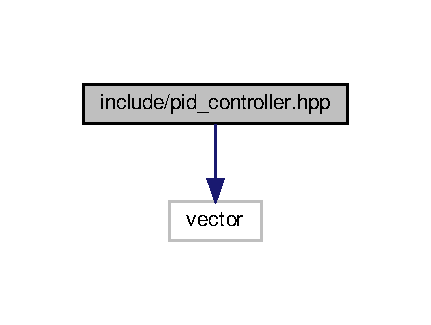
\includegraphics[width=207pt]{pid__controller_8hpp__incl}
\end{center}
\end{figure}
\subsection*{Classes}
\begin{DoxyCompactItemize}
\item 
class \hyperlink{classPIDController}{P\+I\+D\+Controller}
\begin{DoxyCompactList}\small\item\em A class to implement P\+ID controller for velocity. \end{DoxyCompactList}\end{DoxyCompactItemize}


\subsection{Detailed Description}
Header file for \hyperlink{classPIDController}{P\+I\+D\+Controller} class. 

\begin{DoxyAuthor}{Author}
Sakshi Kakde, Hrushikesh Budhale 
\end{DoxyAuthor}
\begin{DoxyVersion}{Version}
0.\+1 
\end{DoxyVersion}
\begin{DoxyDate}{Date}
2021-\/09-\/30
\end{DoxyDate}
\begin{DoxyCopyright}{Copyright}
Copyright (c) 2021 
\end{DoxyCopyright}

%--- End generated contents ---

% Index
\backmatter
\newpage
\phantomsection
\clearemptydoublepage
\addcontentsline{toc}{chapter}{Index}
\printindex

\end{document}
